%
% grundlagen.tex -- Grundlagen
%
% (c) 2021 Prof Dr Andreas Müller, OST Ostschweizer Fachhochschule
%
\section{Matrixpotenzen
\label{buch:section:grundlagen}}
\rhead{Matrixpotenzen}
Die Zerlegung einer Matrix in einfachere Blöcke ist gleichbedeutend
damit, Basen für Unterräume zu finden, die sich unter der Abbildung
nicht ändern.
Im Allgemeinen wird der ganze Raum $\Bbbk^n$ kein solcher invarianter
Unterraum sein.
In diesem Abschnitt soll gezeigt werden, wie man durch Iteration
der Abbildung, also durch Betrachtung von Matrixpotenzen, immer zu
\index{Matrixpotenz}%
einer Zerlegung in invariante Unterräume kommen kann.
\index{invarianter Unterraum}%
\index{Unterraum, invarianter}%
Daraus ergibt sich dann in Abschnitt~\ref{buch:subsection:nilpotente-matrizen}
bereits eine Normalform für nilpotente Matrizen.
\index{nilpotent}%

\begin{figure}
\centering
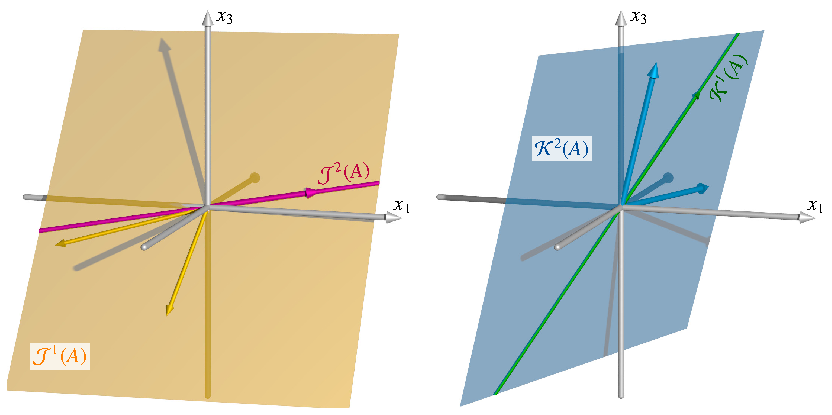
\includegraphics[width=\textwidth]{chapters/40-eigenwerte/images/kernbild.pdf}
\caption{Iterierte Kerne und Bilder einer $3\times 3$-Matrix mit Rang~2.
Die abnehmend geschachtelten iterierten Bilder
$\mathcal{J}^1(A) \subset \mathcal{J}^2(A)$
sind links dargestellt, die zunehmend geschachtelten iterierten Kerne
$\mathcal{K}^1(A) \subset \mathcal{K}^2(A)$ rechts.
\label{buch:eigenwerte:img:kernbild}}
\end{figure}

\begin{figure}
\centering
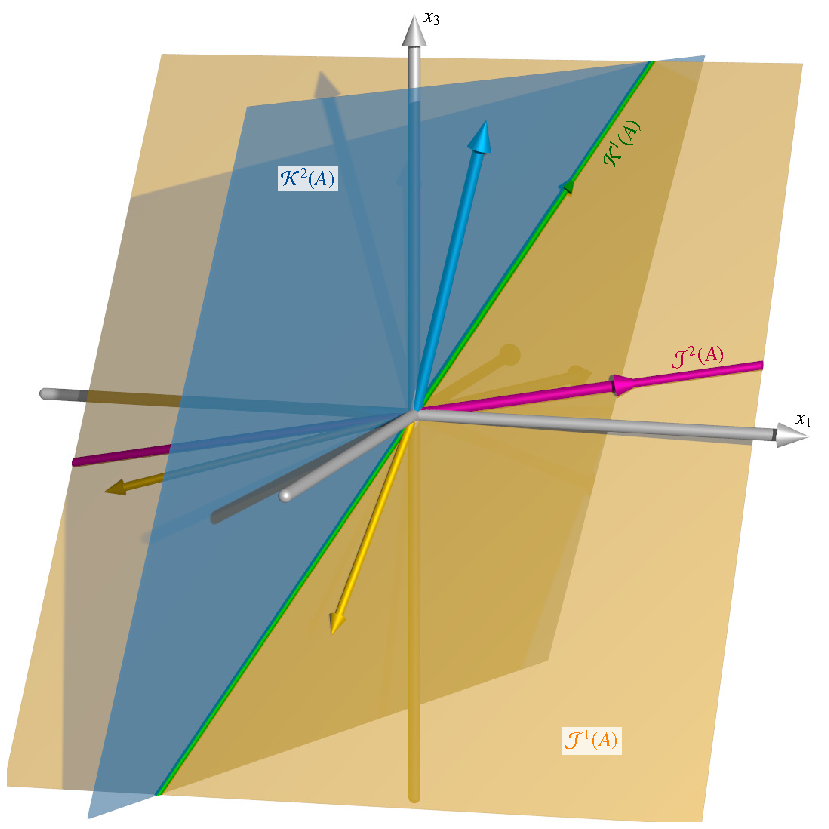
\includegraphics[width=\textwidth]{chapters/40-eigenwerte/images/kombiniert.pdf}
\caption{Iterierte Kerne und Bilder einer $3\times 3$-Matrix mit Rang~2.
Da $\dim\mathcal{J}^2(A)=1$ und $\dim\mathcal{J}^1(A)=2$ ist, muss es
einen Vektor in $\mathcal{J}^1(A)$ geben, der von $A$ auf $0$ abgebildet
wird, der also auch im Kern $\mathcal{K}^1(A)$ liegt.
Daher ist $\mathcal{K}^1(A)$ die Schnittgerade von $\mathcal{J}^1(A)$ und
$\mathcal{K}^2(A)$.
Man kann auch gut erkennen, dass
$\mathbb{R}^3
=
\mathcal{K}^1(A)\oplus \mathcal{J}^1(A)
=
\mathcal{K}^2(A) \oplus \mathcal{J}^2(A)$
ist.
\label{buch:eigenwerte:img:kombiniert}}
\end{figure}

%
% Kern und Bild von Matrixpotenzen
%
\subsection{Kern und Bild von Matrixpotenzen
\label{buch:subsection:kern-und-bild}}
In diesem Abschnitt ist $A\in M_n(\Bbbk)$, $A$ beschreibt eine lineare
Abbildung $f\colon\Bbbk^n\to \Bbbk^n$.
Im Folgenden sollen Kern und Bild der Potenzen $A^k$ untersucht werden.
\begin{definition}
Wir bezeichnen Kern und Bild der iterierten Abbildung $A^k$ mit
\[
\mathcal{K}^k(A)
=
\ker A^k
\qquad\text{und}\qquad
\mathcal{J}^k(A)
=
\operatorname{im} A^k.
\]
\index{KkA@$\mathcal{K}^k(A)$}%
\index{JkA@$\mathcal{J}^k(A)$}%
\end{definition}

Durch Iteration wird das Bild immer kleiner.
Wegen
\[
\mathcal{J}^k (A)
=
\operatorname{im} A^k
=
\operatorname{im} A^{k-1} A
=
\{ A^{k-1} Av\;|\; v \in \Bbbk^n\}
\subset
\{ A^{k-1} v\;|\; v \in \Bbbk^n\}
=
\mathcal{J}^{k-1}(A)
\]
folgt
\begin{equation}
\Bbbk^n
=
\operatorname{im}E
=
\operatorname{im}A^0
=
\mathcal{J}^0(A)
\supset
\mathcal{J}^1(A)
=
\operatorname{im}A
\supset
\mathcal{J}^2(A)
\supset\dots\supset
\mathcal{J}^k(A)
\supset
\mathcal{J}^{k+1}(A)
\supset \dots \supset
\{0\}.
\label{buch:eigenwerte:eqn:Jkchain}
\end{equation}
Für die Kerne gilt etwas Ähnliches, sie werden immer grösser.
Ein Vektor $x\in \mathcal{K}^k(A)$ erfüllt $A^kx=0$.
Dann erfüllt er aber erst recht auch
\[
A^{k+1}x=A\underbrace{A^kx}_{\displaystyle=0}=0,
\]
also ist $x\in\mathcal{K}^k(A)$.
Es folgt
\begin{equation}
\{0\}
=
\mathcal{K}^0(A) = \ker A^0 = \ker E
\subset
\mathcal{K}^1(A) = \ker A
\subset
\dots
\subset
\mathcal{K}^k(A)
\subset
\mathcal{K}^{k+1}(A)
\subset
\dots
\subset
\Bbbk^n.
\label{buch:eigenwerte:eqn:Kkchain}
\end{equation}
Neben diesen offensichtlichen Resultaten kann man aber noch mehr
sagen.
Es ist klar, dass in beiden Ketten
\label{buch:eigenwerte:eqn:Jkchain}
und
\label{buch:eigenwerte:eqn:Kkchain}
nur in höchstens $n$ Schritten eine wirkliche Änderung stattfinden 
kann.
Man kann aber sogar genau sagen, wo Änderungen stattfinden:

\begin{satz}
\label{buch:eigenwerte:satz:ketten}
Ist $A\in M_n(\Bbbk)$ eine $n\times n$-Matrix, dann gibt es eine Zahl $k$
so, dass
\[
\begin{array}{rcccccccccccl}
0=\mathcal{K}^0(A)
&\subsetneq& \mathcal{K}^1(A) &\subsetneq& \mathcal{K}^2(A)
&\subsetneq&\dots&\subsetneq&
\mathcal{K}^k(A) &=& \mathcal{K}^{k+1}(A) &=& \dots
\\
\Bbbk^n= \mathcal{J}^0(A)
&\supsetneq& \mathcal{J}^1(A) &\supsetneq& \mathcal{J}^2(A)
&\supsetneq&\dots&\supsetneq&
\mathcal{J}^k(A) &=& \mathcal{J}^{k+1}(A) &=& \dots
\end{array}
\]
ist.
\end{satz}

\begin{proof}[Beweis]
Es sind zwei Aussagen zu beweisen.
Erstens müssen wir zeigen, dass die Dimension von $\mathcal{K}^i(A)$ 
nicht mehr grösser werden kann, wenn sie zweimal hintereinander gleich war.
Nehmen wir daher an, dass $\mathcal{K}^i(A) = \mathcal{K}^{i+1}(A)$.
Wir müssen $\mathcal{K}^{i+2}(A)$ bestimmen.
$\mathcal{K}^{i+2}(A)$ besteht aus allen Vektoren $x\in\Bbbk^n$ derart,
dass $Ax\in \mathcal{K}^{i+1}(A)=\mathcal{K}^i(A)$ ist.
Daraus ergibt sich, dass $AA^ix=0$, also ist $x\in\mathcal{K}^{i+1}(A)$.
Wir erhalten also
$\mathcal{K}^{i+2}(A)\subset\mathcal{K}^{i+1}\subset\mathcal{K}^{i+2}(A)$,
dies ist nur möglich, wenn beide gleich sind.

Analog kann man für die Bilder vorgehen.
Wir nehmen an, dass $\mathcal{J}^i(A) = \mathcal{J}^{i+1}(A)$ und
bestimmten $\mathcal{J}^{i+2}(A)$.
$\mathcal{J}^{i+2}(A)$ besteht aus all jenen Vektoren, die als
$Ax$ mit $x\in\mathcal{J}^{i+1}(A)=\mathcal{J}^i(A)$ erhalten
werden können.
Es gibt also insbesondere ein $y\in\Bbbk^n$ mit $x=A^iy$.
Dann ist $Ax=A^{i+1}y\in\mathcal{J}^{i+1}(A)$.
Insbesondere besteht $\mathcal{J}^{i+2}(A)$ genau aus den Vektoren
von $\mathcal{J}^{i+1}(A)$.

Zweitens müssen wir zeigen, dass die beiden Ketten bei der gleichen
Potenz von $A$ konstant werden.
Dies folgt jedoch daraus, dass $\dim\mathcal{J}^i(A) = \operatorname{Rang} A^i
= n - \dim\ker A^i = n -\dim\mathcal{K}^i(A)$.
Der Raum $\mathcal{J}^k(A)$ hört also beim gleichen $i$ auf, kleiner
zu werden, bei dem auch $\mathcal{K}^i(A)$ aufhört, grösser zu werden.
\end{proof}

\begin{satz}
Die Zahl $k$ in Satz~\ref{buch:eigenwerte:satz:ketten}
ist nicht grösser als $n$, also
\[
\mathcal{K}^n(A) = \mathcal{K}^l(A)
\qquad\text{und}\qquad
\mathcal{J}^n(A) = \mathcal{J}^l(A)
\]
für $l\ge n$.
\end{satz}

\begin{proof}[Beweis]
Nach Satz~\ref{buch:eigenwerte:satz:ketten} muss die
Dimension von $\mathcal{K}^i(A)$ in jedem Schritt um mindestens
$1$ zunehmen, das ist nur möglich, bis zur Dimension $n$.
Somit können sich $\mathcal{K}^i(A)$ und $\mathcal{J}^i(A)$ für $i>n$
nicht mehr ändern.
\end{proof}

\begin{figure}
\centering
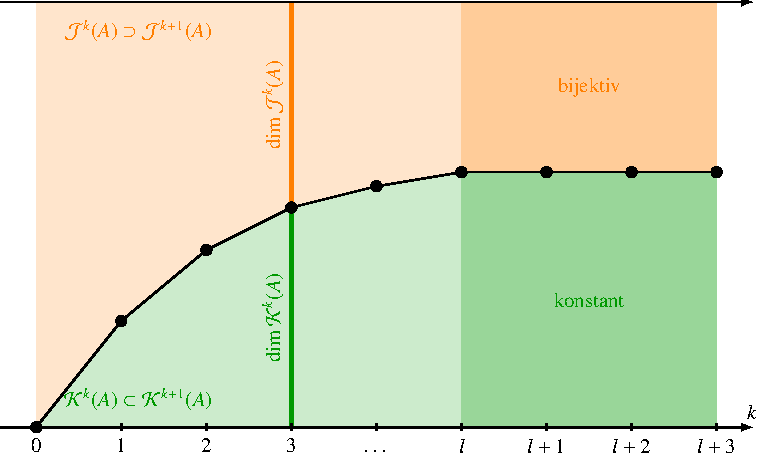
\includegraphics{chapters/40-eigenwerte/images/dimjk.pdf}
\caption{Entwicklung der Dimension von $\dim\mathcal{K}^k(A)$ (grün)
und $\dim\mathcal{J}^k(A)$ (orange) in Abhängigkeit vom Exponenten $k$.
Für $k\ge l$ ändern sich die Dimensionen nicht mehr, $A$ eingeschränkt
auf $\mathcal{J}^l(A)=\mathcal{J}(A)$ ist injektiv.
\label{buch:eigenwerte:fig:dimjk}}
\end{figure}

Abbildung~\ref{buch:eigenwerte:fig:dimjk} zeigt die Abhängigkeit der
Dimensionen $\dim\mathcal{K}^k(A)$ und $\dim\mathcal{J}^k(A)$ von $k$.
Die Dimension $\dim\mathcal{J}^k(A)$ nimmt ab bis zu $k=l$, danach ändert
sie sich nicht mehr und die Einschränkung von $A$ auf $\mathcal{J}^l(A)$ 
ist injektiv.
Die Dimension $\dim\mathcal{K}^k(A)$ nimmt zu bis zu $k=l$, danach
ändert sie sich nicht mehr.

\begin{definition}
\label{buch:eigenwerte:def:KundJ}
Die gemäss Satz~\ref{buch:eigenwerte:satz:ketten} identischen Unterräume
$\mathcal{K}^i(A)$ für $i\ge k$ und die identischen Unterräume
$\mathcal{J}^i(A)$ für $i\ge k$ werden mit
\[
\begin{aligned}
\mathcal{K}(A) &= \mathcal{K}^i(A)&&\forall i\ge k \qquad\text{und}
\\
\mathcal{J}(A) &= \mathcal{J}^i(A)&&\forall i\ge k
\end{aligned}
\]
\index{KA@$\mathcal{K}(A)$}
\index{JA@$\mathcal{J}(A)$}
bezeichnet.
\end{definition}


%
% Inveriante Unterräume
%
\subsection{Invariante Unterräume
\label{buch:subsection:invariante-unterraeume}}
Kern und Bild sind der erste Schritt zu einem besseren Verständnis 
einer linearen Abbildung oder ihrer Matrix.
Invariante Räume dienen dazu, eine lineare Abbildung in einfachere
Abbildungen zwischen ``kleineren'' Räumen zu zerlegen, wo sie leichter
analysiert werden können.

\begin{definition}
\label{buch:eigenwerte:def:invarianter-unterraum}
Sei $f\colon V\to V$ eine lineare Abbildung eines Vektorraums in sich
selbst.
Ein Unterraum $U\subset V$ heisst {\em invarianter Unterraum},
wenn
\[
f(U) = \{ f(x)\;|\; x\in U\} \subset U
\]
gilt.
\index{invarianter Unterraum}%
\index{Unterraum, invarianter}%
\end{definition}

Der Kern $\ker A$  einer linearen Abbildung ist trivialerweise ein
invarianter Unterraum, da alle Vektoren in $\ker A$ auf $0\in\ker A$
abgebildet werden.
Ebenso ist natürlich $\operatorname{im}A$ ein invarianter Unterraum,
denn jeder Vektor wird in $\operatorname{im}A$ abgebildet, insbesondere
auch jeder Vektor in $\operatorname{im}A$.

\begin{satz}
\label{buch:eigenwerte:satz:KJinvariant}
Sei $f\colon V\to V$ eine lineare Abbildung mit Matrix $A$.
Jeder der Unterräume $\mathcal{J}^i(A)$ und $\mathcal{K}^i(A)$ 
ist ein invarianter Unterraum.
\end{satz}

\begin{proof}[Beweis]
Sei $x\in\mathcal{K}^i(A)$, es gilt also $A^ix=0$.
Wir müssen überprüfen, dass $Ax\in\mathcal{K}^i(A)$.
Wir berechnen daher $A^i\cdot Ax=A^{i+1}x=A\cdot A^ix = A\cdot 0=0$,
was zeigt, dass $Ax\in\mathcal{K}^i(A)$.

Sei jetzt $x\in\mathcal{J}^i(A)$, es gibt also ein $y\in V$ derart, dass
$A^iy=x$.
Wir müssen überprüfen, dass $Ax\in\mathcal{J}^i(A)$.
Dazu berechnen wir $Ax=AA^iy=A^iAy\in\mathcal{J}^i(A)$, $Ax$ ist also das
Bild von $Ay$ unter $A^i$.
\end{proof}

\begin{korollar}
Die Unterräume $\mathcal{K}(A)\subset V$ und $\mathcal{J}(A)\subset V$
sind invariante Unterräume.
\end{korollar}

Die beiden Unterräume $\mathcal{K}(A)$ und $\mathcal{J}(A)$ sind besonders
interessant, da wir aus der Einschränkung der Abbildung $f$ auf diese
Unterräume mehr über $f$ lernen können.

\begin{satz}
\label{buch:eigenwerte:satz:fJinj}
Die Einschränkung von $f$ auf $\mathcal{J}(A)$ ist injektiv.
\end{satz}

\begin{proof}[Beweis]
Die Einschränkung von $f$ auf $\mathcal{J}^k(A)$ ist
$\mathcal{J}^k(A) \to \mathcal{J}^{k+1}(A)$, nach Definition von
$\mathcal{J}^{k+1}(A)$ ist diese Abbildung surjektiv.
Da aber $\mathcal{J}^k(A)=\mathcal{J}^{k+1}(A)$ ist, ist
$f\colon \mathcal{J}^k(A)\to\mathcal{J}^k(A)$ surjektiv,
also ist $f$ auf $\mathcal{J}^k(A)$ auch injektiv.
\end{proof}

Die beiden Unterräume $\mathcal{J}(A)$ und $\mathcal{K}(A)$
sind Bild und Kern der iterierten Abbildung mit Matrix $A^k$.
Das bedeutet, dass $\dim\mathcal{J}(A)+\mathcal{K}(A)=n$.
Da $\mathcal{K}(A)=\ker A^k$ und andererseits $A$ injektiv ist auf
$\mathcal{J}(A)$, muss $\mathcal{J}(A)\cap\mathcal{K}(A)=0$.
Es folgt, dass $V=\mathcal{J}(A) + \mathcal{K}(A)$.

In $\mathcal{K}(A)$ und $\mathcal{J}(A)$ kann man unabhängig voneinander
jeweils eine Basis wählen.
Die Basen von $\mathcal{K}(A)$ und $\mathcal{J}(A)$ zusammen ergeben
eine Basis von $V$.
Die Matrix $A'$ in dieser Basis wird die Blockform
\[
A'
=
\left(
\begin{array}{ccc|ccc}
&&&&&\\
&A'_{\mathcal{K}}&&&&\\
&&&&&\\
\hline
&&&&&\\
&&&&A'_{\mathcal{J}}&\\
&&&&&\\
\end{array}
\right)
\]
haben, wobei die Matrix $A_\mathcal{J}'$ invertierbar ist.
Die Zerlegung in invariante Unterräume ergibt also eine natürlich
Aufteilung der Matrix $A$ in kleiner Matrizen mit zum Teil bekannten
Eigenschaften.

%
% Spezialfall, nilpotente Matrizen
%
\subsection{Nilpotente Matrizen
\label{buch:subsection:nilpotente-matrizen}}
Die Zerlegung von $V$ in die beiden invarianten Unterräume $\mathcal{J}(A)$
und $\mathcal{K}(A)$ reduziert die lineare Abbildung auf zwei Abbildungen
mit speziellen Eigenschaften.
Es wurde bereits in Satz~\label{buch:eigenwerte:satz:fJinj} gezeigt,
dass die Einschränkung auf $\mathcal{J}(A)$ injektiv ist.
Die Einschränkung auf $\mathcal{K}(A)$ bildet nach
Definition~\ref{buch:eigenwerte:def:KundJ} alle
Vektoren nach $k$-facher Iteration auf $0$ ab, $A^k\mathcal{K}(A)=0$.
Solche Abbildungen haben eine speziellen Namen.

\begin{definition}
\label{buch:eigenwerte:def:nilpotent}
Eine Matrix $A$ heisst {\em nilpotent}, wenn es eine Zahl $k$ gibt, so dass
$A^k=0$.
\index{nilpotent}%
\end{definition}

\begin{beispiel}
Obere (oder untere) Dreiecksmatrizen mit Nullen auf der Diagonalen
sind nilpotent.
\index{Dreiecksmatrix}%
Wir rechnen dies wie folgt nach.
Die Matrix $A$ mit Einträgen $a_{i\!j}$
\[
A=\begin{pmatrix}
  0   &a_{12}&a_{13}&\dots &a_{1,n-1}&a_{1n}   \\
  0   &  0   &a_{23}&\dots &a_{1,n-1}&a_{2n}   \\
  0   &  0   &  0   &\dots &a_{1,n-1}&a_{3n}   \\
\vdots&\vdots&\vdots&\ddots&\vdots   &\vdots   \\
  0   &  0   &  0   &\dots &  0      &a_{n-1,n}\\
  0   &  0   &  0   &\dots &  0      &  0
\end{pmatrix}
\]
erfüllt $a_{i\!j}=0$ für $i\ge j$.
Wir zeigen jetzt, dass sich bei der Multiplikation die nicht
verschwinden Elemente bei der Multiplikation noch rechts oben
verschieben.
Dazu multiplizieren wir zwei Matrizen $B$ und $C$ mit
$b_{i\!j}=0$ für $i+k>j$ und $c_{i\!j}=0$ für $i+l>j$.
In der folgenden graphischen Darstellung der Matrizen sind die
Bereiche, wo die Matrixelemente verschwinden, weiss.
\begin{center}
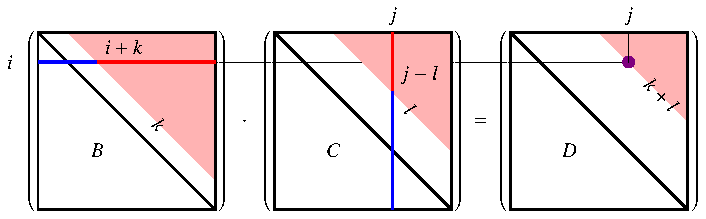
\includegraphics{chapters/40-eigenwerte/images/nilpotent.pdf}
\end{center}
Bei der Berechnung des Elementes $d_{i\!j}$ wird die Zeile $i$ von $B$
mit der Spalte $j$ von $C$ multipliziert.
Die blau eingefärbten Elemente in dieser Zeile und Spalte sind $0$.
Aus der Darstellung ist abzulesen, dass das Produkt verschwindet, 
wenn die roten, von $0$ verschiedenen Elemente von den blauen
Elementen annihiliert werden.
Dies passiert immer, wenn $i+k>j-l$ ist, oder $i+(k+l)> j$.

Wir wenden diese Beobachtung jetzt auf die Potenzen $A^s$ an.
Für die Matrixelemente von $A^s$ schreiben wir $a^s_{i\!j}$.
Wir behaupten, dass die Matrixelemente von $A^s$ die Bedingung
$a_{i\!j}^s=0$ für $i+s>j$ erfüllen.
Dies ist für $s=1$ nach Voraussetzung richtig, dies ist die
Induktionsverankerung.
Nehmen wir jetzt an, dass $a_{i\!j}^s=0$ für $i+s>j$, dann folgt
aus obiger Rechnung, dass $a_{i\!j}^{s+1}=0$ für $i+s+1>j$, so
dass die Bedingung auch für $A^s$ gilt (Induktionsschritt).
Mit vollständiger Induktion folgt, dass $a_{i\!j}^s=0$ für $i+s>j$.
Insbesondere ist $A^n=0$, die Matrix $A$ ist nilpotent.
\end{beispiel}


Man kann die Konstruktion der Unterräume $\mathcal{K}^i(A)$ weiter
dazu verwenden, eine Basis zu finden, in der eine nilpotente Matrix
eine besonders einfach Form erhält.

\begin{satz}
\label{buch:eigenwerte:satz:nnilpotent}
Sei $A$ eine nilpotente $n\times n$-Matrix mit der Eigenschaft, dass
$A^{n-1}\ne 0$.
Dann gibt es eine Basis so, dass $A$ die Form
\begin{equation}
A'
=
\begin{pmatrix}
0&1& &      & & \\
 &0&1&      & & \\
 & &0&      & & \\
 & & &\ddots&1& \\
 & & &      &0&1\\
 & & &      & &0\\
\end{pmatrix}
\label{buch:eigenwerte:eqn:nnilpotent}
\end{equation}
bekommt.
\end{satz}

\begin{proof}[Beweis]
Da $A^{n-1}\ne 0$ ist, gibt es einen Vektor $b_n$ derart, dass $A^{n-1}b_n\ne0$.
Wir konstruieren die Vektoren
\[
b_n,\;
b_{n-1}=Ab_n,\;
b_{n-2}=Ab_{n-1},\;
\dots,\;
b_2=Ab_3,\;
b_1=Ab_2.
\]
Aus der Konstruktion folgt $b_1=A^{n-1}b_n\ne 0$, aber $Ab_1=A^nb_n=0$.
Aus der Konstruktion der iterierten Kerne $\mathcal{K}^i(A)$ folgt jetzt,
dass die Vektoren $b_1,\dots,b_n$ eine Basis bilden.
In dieser Basis hat die Matrix die Form~\ref{buch:eigenwerte:eqn:nnilpotent}.
\end{proof}

\begin{definition}
Wir bezeichnen mit $N_n$ eine Matrix der Form
\eqref{buch:eigenwerte:eqn:nnilpotent}.
\end{definition}

Mit etwas mehr Sorgfalt kann man auch die Bedingung, dass $A^{n-1}\ne 0$
sein muss, im Satz~\ref{buch:eigenwerte:satz:nnilpotent} loswerden.
Sie bedeutet nämlich dass sich die Matrix in mehrere kleinere Blöcke
der Form~\eqref{buch:eigenwerte:eqn:nnilpotent} zerlegen lässt, wie
der folgende Satz zeigt.

\begin{satz}
\label{buch:eigenwerte:satz:allgnilpotent}
Sei $A$ ein nilpotente Matrix, dann gibt es eine Basis, in der die Matrix
aus lauter Nullen besteht ausser in den Einträgen unmittelbar oberhalb der 
Hauptdiagonalen, wo die Einträge $0$ oder $1$ sind.
Insbesondere zerfällt eine solche Matrix in Blöcke der Form $N_{k_i}$,
$i=1,\dots,l$,
wobei $k_1+\dots+k_l=n$ sein muss:
\begin{equation}
\def\temp#1{\multicolumn{1}{|c}{\raisebox{0pt}[17pt][12pt]{\phantom{x}$#1\mathstrut$}\phantom{x}}}
A'
=\left(
\begin{array}{cccc}
\cline{1-1}
\temp{N_{k_1}} &\multicolumn{1}{|c}{}&        &           \\
\cline{1-2}
          &\temp{N_{k_2}}&\multicolumn{1}{|c}{}&           \\
\cline{2-3}
          &           &\temp{\ddots}&\multicolumn{1}{|c}{}\\
\cline{3-4}
          &           &        &\multicolumn{1}{|c|}{\raisebox{0pt}[17pt][12pt]{\phantom{x}$N_{k_l}$}\phantom{x}}\\
\cline{4-4}
\end{array}
\right).
\label{buch:eigenwerte:eqn:allgnilpotent}
\end{equation}
\end{satz}

Im Abschnitt~\ref{buch:subsection:normalform-einer-nilpotenten-matrix}
wird ein Algorithmus zur Bestimmung einer geeigneten Basis für die
Normalform~\eqref{buch:eigenwerte:eqn:allgnilpotent} in etwas mehr
Detail dargestellt.

Aus Satz lässt sich für eine beliebige lineare Abbildung auch bereits eine
partielle Normalform finden.
Die Einschränkung von $f$ auf den invarianten Unterraum $\mathcal{K}(A)$
ist nilpotent.
Die Zerlegung $V=\mathcal{J}(A)\oplus \mathcal{K}(A)$ führt also zu einer
Zerlegung der Abbildung $f$ in eine invertierbare Abbildung
$\mathcal{J}(A)\to\mathcal{J}(A)$ und eine
nilpotente Abbildung $\mathcal{K}(A)\to\mathcal{K}(A)$.
Nach Satz~\ref{buch:eigenwerte:satz:allgnilpotent} kann man in
$\mathcal{K}(A)$ eine Basis so wählen, dass die Matrix die Blockform
\eqref{buch:eigenwerte:eqn:allgnilpotent} erhält.


\begin{figure}
\centering
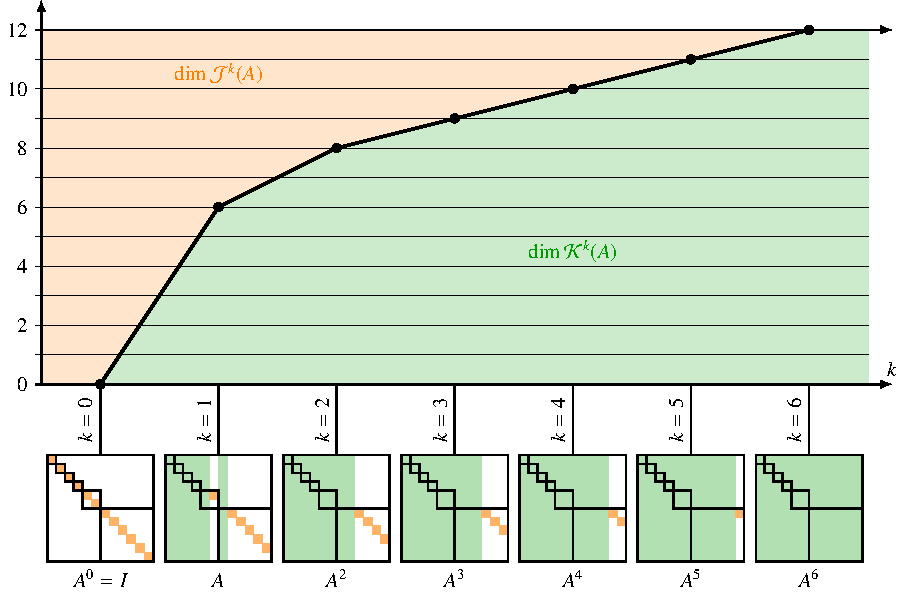
\includegraphics[width=\textwidth]{chapters/40-eigenwerte/images/jknilp.pdf}
\caption{Entwicklung der Dimensionen von Kern und Bild von $A^k$ in
Abhängigkeit von $k$
\label{buch:eigenwte:fig:jknilp}}
\end{figure}

\begin{beispiel}
In der Abbildung~\ref{buch:eigenwte:fig:jknilp} sind die Dimensionen
von Kern und Bild der Matrix
\[
\setcounter{MaxMatrixCols}{12}
A=\begin{pmatrix}
0& & & & & & & & & & & \\
 &0& & & & & & & & & & \\
 & &0& & & & & & & & & \\
 & & &0& & & & & & & & \\
 & & & &0&1& & & & & & \\
 & & & & &0& & & & & & \\
 & & & & & &0&1& & & & \\
 & & & & & & &0&1& & & \\
 & & & & & & & &0&1& & \\
 & & & & & & & & &0&1& \\
 & & & & & & & & & &0&
\end{pmatrix}
\]
dargestellt.
Die Matrix $A^k$ ist in den kleinen Quadraten am unteren Rand der Matrix
symbolisch dargestellt.
Grüne Spalten bestehen aus lauter Nullen, die zugehörigen
Standardbasisvektoren werden von diesem $A^k$ auf $0$ abgebildet.
Die orangen Felder enthalten Einsen, die entsprechenden Standardbasisvektoren
bilden daher eine Basis des Bildes von $A^k$.
\end{beispiel}

%
% Basis für die Jordan-Normalform einer nilpotenten Matrix
%
\subsection{Basis für die Normalform einer nilpotenten Matrix bestimmen
\label{buch:subsection:normalform-einer-nilpotenten-matrix}}
Die Zerlegung in die invarianten Unterräume $\mathcal{J}^k(f)$ und
$\mathcal{K}^k(f)$ ermöglichen, eine Basis zu finden, in der die
Matrix von $f$ die Blockform \eqref{buch:eigenwerte:eqn:allgnilpotent}
hat.
In diesem Abschnitt soll die Konstruktion einer solchen Basis
etwas ausführlicher beschrieben werden.

\begin{figure}
\centering
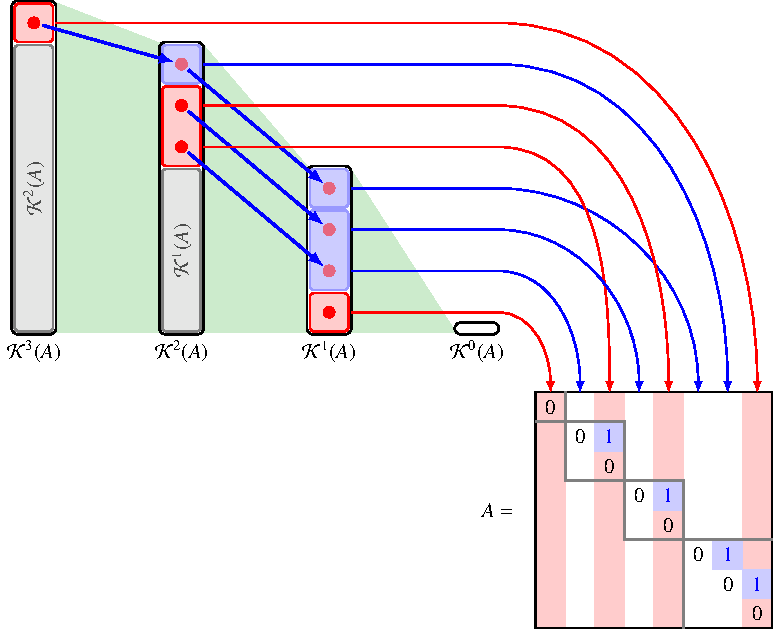
\includegraphics{chapters/40-eigenwerte/images/normalform.pdf}
\caption{Konstruktion der Basis für die Jordansche Normalform einer
nilpotenten Matrix.
Die Vektoren werden in der Reihenfolge von rechts nach links in die
Matrix gefüllt.
\label{buch:eigenwerte:fig:normalform}}
\end{figure}

Abbildung~\ref{buch:eigenwerte:fig:normalform} illustriert den Prozess
an einer nilpotenten Matrix $A$ mit $A^3=0$
Die vertikalen Rechtecke im linken Teil der Abbildung symbolisieren
die Unterräume $\mathcal{K}^k(A)$.
Es ist bekannt, dass $\mathcal{K}^k(A) \subset \mathcal{K}^{k+1}(A)$ ist,
die Einbettung wird in der Abbildung durch graue Rechtecke dargestellt.
Es sei wieder $l$ der Exponent, für den $\mathcal{K}^l(A)=\Bbbk^n$ wird.
Da $\mathcal{K}^{l-1}(A)\ne \mathcal{K}^l(A)$ ist, muss es einen
komplementären Unterraum geben, in dem eine Basis gewählt wird.
Jeder der Vektoren $b_1,\dots,b_s$ dieser Basis gibt Anlass zu einem
Block der Form $N_l$, der auf dem Unterraum 
$\langle b_i,Ab_i,\dots,A^{l-1}b_i\rangle$ operiert.
In der Abbildung ist $b_i$ durch einen roten Punkt symbolisiert und
die Bilder $Ab_i,\dots,A^{l-1}b_i$ werden durch blaue Pfeile untereinander
verbunden.

Der Raum $\mathcal{K}^{l-1}(A)$ enthält dann $\mathcal{K}^{l-2}(A)$ und
die Vektoren $Ab_1,\dots,Ab_s$.
Es ist aber möglich, dass diese Vektoren nicht den ganzen Raum
$\mathcal{K}^{l-1}(A)$ erzeugen.
In diesem Fall lassen sich die Vektoren mit Hilfe weiterer Vektoren
$b_{s+1},\dots,b_{s+r}$ zu einer Basisi von $\mathcal{K}^{l-1}(A)$
ergänzen.
Wie vorhin gibt jeder der Vektoren $b_{s+i}$ Anlass zu einem Block
der Form $N_{l-1}$, der auf dem Unterraum
$\langle b_{s+i},Ab_{s+i}\dots,A^{l-2}b_{s+i}\rangle$
operiert.

Durch Wiederholung dieses Prozesses können schrittweise Basisvektoren
$b_i$ erzeugt werden.
Die Matrix der Abbildung $f$ in der Basis $\{b_i,Ab_i,\dots,A^kb_i\}$
ist ein Block der Form $N_k$.
Für $0\le k\le l-1$ sind die Vektoren $A^kb_i$,
solange sie von $0$ verschieden sind,
alle nach Konstruktion linear unabhängig, sie bilden eine Basis
von $\mathcal{K}^l(A)=\Bbbk^n$.

\begin{beispiel}
Die Basis für die Zerlegung der Matrix
\[
A
=
\begin{pmatrix*}[r]
  3& 1&-2\\
-21&-7&14\\
 -6&-2& 4
\end{pmatrix*}
\]
in Blockform soll nach der oben beschriebenen Methode ermittelt werden.
Zunächst kann man nachrechnen, dass $A^2=0$ ist.
Der Kern von $A$ ist der Lösungsraum der Gleichung $Ax=0$, da alle Zeilen
Vielfache der ersten Zeile sind, reicht es zu verlangen, dass die
Komponenten $x_i$ der Lösung die Gleichung
\[
3x_1+x_2-2x_3=0
\]
erfüllen.
Jetzt muss ein Vektor $b_1$ ausserhalb von $\mathbb{L}$ gefunden werden,
der erste Standardbasisvektor $e_1$ kann dazu verwendet werden.
Es ist auch klar, dass $Ae_1\ne 0$ ist.
Wir verwenden daher die beiden Vektoren 
\[
b_3=e_1=\begin{pmatrix} 1\\0\\0 \end{pmatrix}
,\qquad
b_2=Ab_3=\begin{pmatrix*}[r] 3\\-21\\-6 \end{pmatrix*}.
\]
In einem Unterraum mit
dieser Basis hat $A$ die Matrix $N_2$.
Jetzt muss noch ein Basisvektor $b_1$ gefunden werden,
der in $\ker A=\mathbb{L}$ liegt und so, dass $b_1$ und $b_2$ 
linear unabhängig sind.
Die zweite Bedingung kann leicht dadurch sichergestellt werden,
dass man die erste Komponente von $b_1$ als $0$ wählt.
Eine mögliche Lösung ist dann
\[
b_1=\begin{pmatrix}0\\2\\1\end{pmatrix}.
\]
Die Matrix 
\[
B=\begin{pmatrix*}[r]
 0& 1&   3\\
 2& 0& -21\\
 1& 0&  -6
\end{pmatrix*}
\qquad\text{mit Inverser}
\qquad
B^{-1}=\begin{pmatrix*}[r]
0&-\frac23& \frac73\\
0&-\frac19& \frac29\\
1& \frac13&-\frac23
\end{pmatrix*}
\]
transformiert die Matrix $A$ auf den Block $N_3$:
\[
B^{-1}AB
=
B^{-1}\begin{pmatrix*}[r]
0&0&  3\\
0&0&-21\\
0&0& -6
\end{pmatrix*}
=
\left(
\begin{array}{c|cc}
0& & \\
\hline
 &0&1\\
 &0&0
\end{array}
\right)
=
N_3.
\qedhere
\]
\end{beispiel}

